% ========================================
%	Header einbinden
% ========================================

\documentclass[bibtotoc,titlepage]{scrartcl}

% Deutsche Spracheinstellungen
\usepackage[ngerman,german]{babel, varioref}
\usepackage[T1]{fontenc}
\usepackage[utf8]{inputenc}

%\usepackage{marvosym}

\usepackage{amsfonts}
\usepackage{amssymb}
\usepackage{amsmath}
\usepackage{amscd}
\usepackage{amstext}
\usepackage{float}
\usepackage{caption}
\usepackage{wrapfig}
\usepackage{setspace}
\usepackage{threeparttable}
\usepackage{footnote}

\usepackage{caption}
\usepackage{subcaption}

\newfloat{formel}{htbp}{for}
\floatname{formel}{Formel}


\usepackage{longtable}

%\usepackage{bibgerm}

\usepackage{footnpag}

\usepackage{ifthen}                 %%% package for conditionals in TeX
\usepackage{siunitx}
%Fr textumflossene Bilder und Tablellen
%\usepackage{floatflt} - veraltet

%Fr Testzwecke aktivieren, zeigt labels und refs im Text an.
%\usepackage{showkeys}

% Abstand zwischen zwei Abs�zen nach DIN (1,5 Zeilen)
% \setlength{\parskip}{1.5ex plus0.5ex minus0.5ex}

% Einrckung am Anfang eines neuen Absatzes nach DIN (keine)
%\setlength{\parindent}{0pt}

% R�der definieren
% \setlength{\oddsidemargin}{0.3cm}
% \setlength{\textwidth}{15.6cm}

% bessere Bildunterschriften
%\usepackage[center]{caption2}


% Probleml�ungen beim Umgang mit Gleitumgebungen
\usepackage{float}

% Nummeriert bis zur Strukturstufe 3 (also <section>, <subsection> und <subsubsection>)
%\setcounter{secnumdepth}{3}

% Fhrt das Inhaltsverzeichnis bis zur Strukturstufe 3
%\setcounter{tocdepth}{3}

\usepackage{exscale}

\newenvironment{dsm} {\begin{displaymath}} {\end{displaymath}}
\newenvironment{vars} {\begin{center}\scriptsize} {\normalsize \end{center}}


\newcommand {\en} {\varepsilon_0}               % Epsilon-Null aus der Elektrodynamik
\newcommand {\lap} {\; \mathbf{\Delta}}         % Laplace-Operator
\newcommand {\R} { \mathbb{R} }                 % Menge der reellen Zahlen
\newcommand {\e} { \ \mathbf{e} }               % Eulersche Zahl
\renewcommand {\i} { \mathbf{i} }               % komplexe Zahl i
\newcommand {\N} { \mathbb{N} }                 % Menge der nat. Zahlen
\newcommand {\C} { \mathbb{C} }                 % Menge der kompl. Zahlen
\newcommand {\Z} { \mathbb{Z} }                 % Menge der kompl. Zahlen
\newcommand {\limi}[1]{\lim_{#1 \rightarrow \infty}} % Limes unendlich
\newcommand {\sumi}[1]{\sum_{#1=0}^\infty}
\newcommand {\rot} {\; \mathrm{rot} \,}         % Rotation
\newcommand {\grad} {\; \mathrm{grad} \,}       % Gradient
\newcommand {\dive} {\; \mathrm{div} \,}        % Divergenz
\newcommand {\dx} {\; \mathrm{d} }              % Differential d
\newcommand {\cotanh} {\; \mathrm{cotanh} \,}   %Cotangenshyperbolicus
\newcommand {\asinh} {\; \mathrm{areasinh} \,}  %Area-Sinus-Hyp.
\newcommand {\acosh} {\; \mathrm{areacosh} \,}  %Area-Cosinus-H.
\newcommand {\atanh} {\; \mathrm{areatanh} \,}  %Area Tangens-H.
\newcommand {\acoth} {\; \mathrm{areacoth} \,}  % Area-cotangens
\newcommand {\Sp} {\; \mathrm{Sp} \,}
\newcommand {\mbe} {\stackrel{\text{!}}{=}}     %Must Be Equal
\newcommand{\qed} { \hfill $\square$\\}
\renewcommand{\i} {\imath}
\def\captionsngerman{\def\figurename{\textbf{Abb.}}}

%%%%%%%%%%%%%%%%%%%%%%%%%%%%%%%%%%%%%%%%%%%%%%%%%%%%%%%%%%%%%%%%%%%%%%%%%%%%
% SWITCH FOR PDFLATEX or LATEX
%%%%%%%%%%%%%%%%%%%%%%%%%%%%%%%%%%%%%%%%%%%%%%%%%%%%%%%%%%%%%%%%%%%%%%%%%%%%
%%%
\ifx\pdfoutput\undefined %%%%%%%%%%%%%%%%%%%%%%%%%%%%%%%%%%%%%%%%% LATEX %%%
%%%
\usepackage[dvips]{graphicx}       %%% graphics for dvips
\DeclareGraphicsExtensions{.eps,.ps}   %%% standard extension for included graphics
\usepackage[ps2pdf]{thumbpdf}      %%% thumbnails for ps2pdf
\usepackage[ps2pdf,                %%% hyper-references for ps2pdf
bookmarks=true,%                   %%% generate bookmarks ...
bookmarksnumbered=true,%           %%% ... with numbers
hypertexnames=false,%              %%% needed for correct links to figures !!!
breaklinks=true,%                  %%% breaks lines, but links are very small
linkbordercolor={0 0 1},%          %%% blue frames around links
pdfborder={0 0 112.0}]{hyperref}%  %%% border-width of frames
%                                      will be multiplied with 0.009 by ps2pdf
%
%\hypersetup{ pdfauthor   = {Hannes Franke; Julius Tilly},
%pdftitle    = {x}, pdfsubject  = {Protokoll FP}, pdfkeywords = {V301, Innenwiderstand, Leistungsanpassung},
%pdfcreator  = {LaTeX with hyperref package}, pdfproducer = {dvips
%+ ps2pdf} }
%%%
\else %%%%%%%%%%%%%%%%%%%%%%%%%%%%%%%%%%%%%%%%%%%%%%%%%%%%%%%%%% PDFLATEX %%%
%%%
\usepackage[pdftex]{graphicx}      %%% graphics for pdfLaTeX
\DeclareGraphicsExtensions{.pdf}   %%% standard extension for included graphics
\usepackage[pdftex]{thumbpdf}      %%% thumbnails for pdflatex
\usepackage[pdftex,                %%% hyper-references for pdflatex
bookmarks=true,%                   %%% generate bookmarks ...
bookmarksnumbered=true,%           %%% ... with numbers
hypertexnames=false,%              %%% needed for correct links to figures !!!
breaklinks=true,%                  %%% break links if exceeding a single line
linkbordercolor={0 0 1},
linktocpage]{hyperref} %%% blue frames around links
%                                  %%% pdfborder={0 0 1} is the default
% \hypersetup{
% pdftitle    = {V301 Innenwiderstand und Leistungsanpassung}, 
% pdfsubject  = {Protokoll AP}, 
% pdfkeywords = {V301, Innenwiderstand, Leistungsanpassung},
% pdfsubject  = {Protokoll AP},
% pdfkeywords = {V301, Innenwiderstand, Leistungsanpassung}}
%                                  %%% pdfcreator, pdfproducer,
%                                      and CreationDate are automatically set
%                                      by pdflatex !!!
\pdfadjustspacing=1                %%% force LaTeX-like character spacing
\usepackage{epstopdf}
%
\fi %%%%%%%%%%%%%%%%%%%%%%%%%%%%%%%%%%%%%%%%%%%%%%%%%%% END OF CONDITION %%%
%%%%%%%%%%%%%%%%%%%%%%%%%%%%%%%%%%%%%%%%%%%%%%%%%%%%%%%%%%%%%%%%%%%%%%%%%%%%
% seitliche Tabellen und Abbildungen
%\usepackage{rotating}
\usepackage{ae}
\usepackage{
  array,
  booktabs,
  dcolumn
}
\makeatletter 
  \renewenvironment{figure}[1][] {% 
    \ifthenelse{\equal{#1}{}}{% 
      \@float{figure} 
    }{% 
      \@float{figure}[#1]% 
    }% 
    \centering 
  }{% 
    \end@float 
  } 
  \makeatother 


  \makeatletter 
  \renewenvironment{table}[1][] {% 
    \ifthenelse{\equal{#1}{}}{% 
      \@float{table} 
    }{% 
      \@float{table}[#1]% 
    }% 
    \centering 
  }{% 
    \end@float 
  } 
  \makeatother 
%\usepackage{listings}
%\lstloadlanguages{[Visual]Basic}
%\allowdisplaybreaks[1]
%\usepackage{hycap}
%\usepackage{fancyunits}

% ========================================
%	Angaben für das Titelblatt
% ========================================

\title{Lehrstuhlversuch E1 - Röntgenreflektometrie\\				% Titel des Versuchs 
	\large TU Dortmund, Fakultät Physik\\ 
	\normalsize Fortgeschrittenen-Praktikum}

\author{Jan Adam\\			% Name Praktikumspartner A
	{\small \href{jan.adam@tu-dortmund.de}{jan.adam@tu-dortmund.de}}	% Erzeugt interaktiven einen Link
	\and						% um einen weiteren Author hinzuzfügen
	Felix Wieland\\					% Name Praktikumspartner B
	{\small \href{felix.wieland@tu-dortmund.de}{felix.wieland@tu-dortmund.de}}		% Erzeugt interaktiven einen Link
}
\date{25.04.2016}				% Das Datum der Versuchsdurchführung

% ========================================
%	Das Dokument beginnt
% ========================================

\begin{document}
	
% ========================================
%	Titelblatt erzeugen
% ========================================

\maketitle					% Jetzt wird die Titelseite erzeugt
\thispagestyle{empty} 				% Weder Kopfzeile noch Fußzeile

% ========================================
%	Der Vorspann
% ========================================

%\newpage					% Wenn Verzeichnisse auf einer neuen Seite beginnen sollen
%\pagestyle{empty}				% Weder Kopf- noch Fußzeile für Verzeichnisse

\tableofcontents

%\newpage					% eine neue Seite
%\thispagestyle{empty}				% Weder Kopf- noch Fußzeile für Verzeichnisse
%\listoffigures					% Abbildungsverzeichnis

%\newpage					% eine neue Seite
%\thispagestyle{empty}				% Weder Kopf- noch Fußzeile für Verzeichnisse
%\listoftables					% Tabellenverzeichnis
\newpage					% eine neue Seite


% ========================================
%	Kapitel
% ========================================
\section{Ziel}
Ziel dieses Versuches ist es das statistische Verhalten und die Bedeutung des elektronischen Rauschens zu untersuchen. Dazu wird zuerst das thermische Rauschen an zwei Widerständen aufgenommen, womit die Boltzmann-Konstante $k_{\textrm{B}}$ berechnet werden kann. Anschließend wird das Schrottrauschen an zwei Elektronenröhren gemessen, um die Elementarladung $e_0$ zu ermitteln und das weit verbreitete $f^{-1}$ Verhalten von Rauschspektren zu untersuchen.

\section{Theoretische Grundlagen}
\subsection{Grundlegende Bemerkungen}
Zur Auswertung von Rauscheffekten werden meistens Mittelwerte herangezogen, da es sich bei Rauscheffekten um stochastische Prozesse handelt. Es lässt sich zeigen, dass für eine Rauschspannung gilt

\begin{align}
\overline{U} = \lim_{\tau \rightarrow \infty} \int_0^\tau U(t)dt = 0 \;,
\label{eqn:Rauschspannung}
\end{align}

wenn man alle Parameter konstant hält, sodass aus der Größe $\overline{U}$ keine weiteren Informationen gewonnen werden können und man stattdessen den quadratischen Mittelwert

\begin{align}
\overline{U^2} = \frac{1}{\tau} \int_0^\tau U^2(t)dt
\label{eqn:quadMittelwert}
\end{align}

betrachtet. Man spricht dabei von stationären Schwankungserscheinungen, sofern $\overline{U^2}$ unabhängig von der Lage des Mittlungszeitintervalls $\tau$ ist.

Das Scharmittel der Rauschspannung

\begin{align}
\langle U^2(t_0) \rangle = \frac{1}{N} \sum_{i=1}^{N} U_i^2(t_0)
\label{eqn:Scharmittel}
\end{align}

ergibt sich durch das Ablesen einer großen Anzahl $N$ von identischen Rauschquellen $U_i(t_0)$ zu einem Zeitpunkt $t_0$. In diesem Fall versteht man unter Stationarität, dass $\langle U^2(t_0) \rangle$ unabhängig von $t_0$ ist. Im Fall $\overline{U^2} = \langle U^2(t_0) \rangle$ bezeichnet man das Rauschen als ergodisch, was sowohl für das thermische Rauschen eines Widerstandes als auch für das Schrotrauschen einer Elektronenröhre der Fall ist.

\subsection{Das thermische Rauschen}
Zur Ableitung eines Zusammenhanges zwischen $\overline{U^2}$ für die Rauschspannung eines thermischen Widerstandes und der Temperatur $T$ geht man von der in Abbildung \ref{FIG:doppelLeitung} dargestelltem Doppelleitung der Länge $L$ aus, die zu Beginn an ihren Enden kurzgeschlossen sein soll und ein schwingungsfähiges System darstellt.

\begin{figure}[htbp]
	\centering
	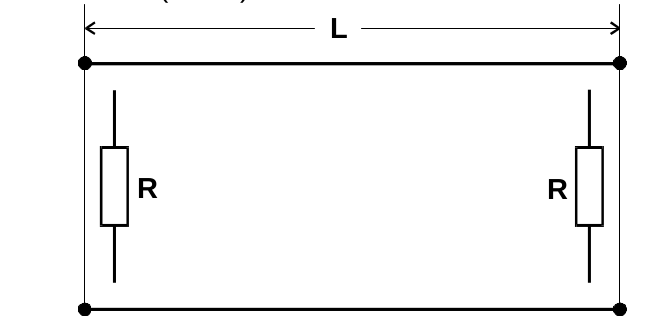
\includegraphics[width=0.5\linewidth,height=0.5\textheight,keepaspectratio]{bilder/doppelLeitung.png}
	\caption{Verlustfreie Doppelleitung. Die Enden sind zu Beginn kurzgeschlossen. Anschließend werden sie durch Widerstände verbunden \cite{Anl}}
	\label{FIG:doppelLeitung}
\end{figure}

Mögliche Eigenschwingungen erfüllen dabei die Gleichung 

\begin{align}
L = n\frac{\lambda}{2}\quad
\end{align}

mit $n \in \mathbb{N}^+$ bzw. mit der Frequenz $\nu$ und der Phasengeschwindigkeit $v$ ausgedrückt

\begin{align}
\nu = n\frac{v}{2L}\;.
\end{align}

Gemäß dem Gleichverteilungssatz der Thermodynamik entfällt auf jede Schwingung der Frequenz $\nu$ die mittlere Energie

\begin{align}
\overline{E} = \frac{h\nu}{\exp\left( \frac{h\nu}{kT}\right) -1}
\end{align}

und die Leistung pro Frequenzintervall $\Delta\nu$ ergibt sich zu

\begin{align}
P = \frac{h\nu}{\exp\left( \frac{h\nu}{kT}\right) -1}\Delta\nu \;.
\end{align}

Werden nun die Enden der Doppelleitung aus Abbildung \ref{FIG:doppelLeitung} mit Widerständen abgeschlossen, so kommt es zu Verlusten in Form von Wärmeabstrahlung. Zur Ausbildung einer stationären Schwingung kann es dann nur kommen, wenn die Energieverluste durch Abstrahlung im zeitlichen Mittel ersetzt werden, was durch Ausbildung einer Rauschspannung $U_{\textrm{R}}$ geschieht.

Zur Berechnung der maximal von der Rauschquelle abgegebenen Leistung setzt man 

\begin{align}
\overline{I^2} = \frac{\overline{U^2}}{R^2+Z^2}
\end{align}

an und erhält somit für die Leistung 

\begin{align}
\overline{N} = \overline{U^2} \frac{Z}{R^2+Z^2} \;,
\end{align}

was im Fall $R = Z$ maximal wird mit dem Wert 

\begin{align}
\overline{N}_{\textrm{max}} = \frac{ \overline{U^2} }{4R} \; .
\end{align}

Im stationären Fall folgt $P = \overline{N}_{\textrm{max}}$ und es lässt sich der Ausdruck

\begin{align}
\overline{U^2}(\nu) = 4RP = 4R \frac{h\nu}{\exp\left( \frac{h\nu}{kT}\right) -1 } \Delta\nu \approx 4kTR\Delta\nu 
\end{align}

aufstellen, der das mittlere Rauschspannungsquadrat $ \overline{U^2}$ eines Widerstandes $R$ bei der Temperatur $T$ im thermodynamischen Gleichgewicht verknüpft. Die Näherung ergibt sich daraus, dass $ 4R \frac{h\nu}{\exp\left( \frac{h\nu}{kT}\right) -1 }$ im Raumtemperaturbereich bis zu Frequenzen von ca. $10^{12}\;$Hz nahezu konstant ist, wie in Abbildung \ref{FIG:frequenzAbh} dargestellt. 

\begin{figure}[htbp]
	\centering
	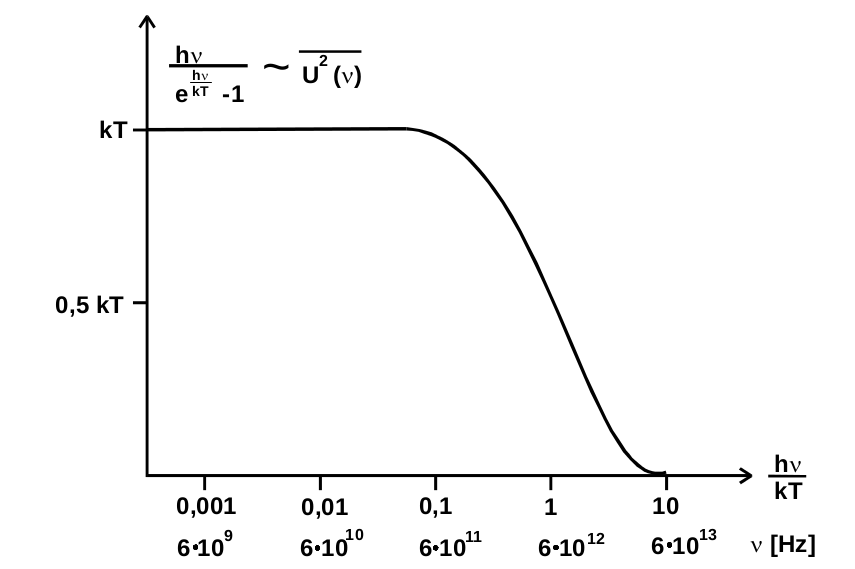
\includegraphics[width=0.65\linewidth,height=0.5\textheight,keepaspectratio]{bilder/frequenzAbh.png}
	\caption{Schematisch Darstellung der Frequenzabhängigkeit der Rauschspannung an einem ohmschen Widerstand \cite{Anl}}
	\label{FIG:frequenzAbh}
\end{figure}

Für $h\nu \ll kT$ nähert man

\begin{align}
\exp\left( \frac{h\nu}{kT} \right) = 1 + \frac{h\nu}{kT} + \ldots \;.
\end{align}

Die sogenannte Nyquist-Beziehung 

\begin{align}
\overline{U^2}(\nu) = 4kTR\Delta\nu \label{eqn:Nyquist}
\end{align}

ist nur noch von der Breite des durch die Messapparatur vorgegebenen Frequenzbereiches, aber nicht von der Lange auf der Frequenzskala abhängig, weswegen man von weißem Rauschen spricht.

Da die verwendeten Kabel über Kapazitätsbelage verfügen wirken sie wie ein RC-Tiefpass und die gemessene Spannung $\overline{U^2}_{\textrm{RC}}$ ist gegenüber $\overline{U^2}(\nu)$ um einen Faktor

\begin{align}
\overline{U^2}_{\textrm{RC}}(\nu) = \overline{U^2}(\nu) \frac{1}{1 + \left(2\pi\nu{}RC\right)^2} \;. \label{eqn:NyquistRC}
\end{align}

verringert.

\subsection{Das Schrotrauschen einer Metallkatode und die Schottky-Beziehung}
\label{sec:Schrotrauschen}
Der Schroteffekt lässt sich am besten an einer Vakuumdiode mit einer Reinmetallkathode, die im Sättigungsbereich betrieben wird, untersuchen, sodass alle emittierten Elektronen die Anode erreichen. Der gemessene Strom $I_{\textrm{Ges}} = I_0 + I(t)$ setzt sich aus einem konstantem Anteil $I_0$ und einem Rauschstromanteil $I(t)$ zusammen, wobei $\overline{I}(t) = 0$ gilt. Zur Berechnung des mittleren Rauschstromquadrates $\overline{I^2}$ werden Annahmen eingeführt, die aber im Sättigungsbetrieb erfüllt sind:

\begin{enumerate}
	\item Die Elektronen werden unabhängig voneinander von der Glühkathode emittiert
	\item Die Bewegung der Elektronen ist unabhängig voneinander, sodass keine Raumladungen vorhanden sein dürfen und die Anodenspannung ausreichend hoch gewählt werden muss.
	\item Die Elektronen haben nahezu keine Anfangsgeschwindigkeit nach Austritt aus der Glühkathode.
	\item Die Elektronen haben den gleichen Weg-Zeit-Verlauf.
	\item Die Elektronen lösen keine Sekundärelektronen an der Anode aus.
\end{enumerate}

Ein einzelnes sich von der Kathode zur Anode bewegendes Elektron ruft während seiner Laufzeit $\tau$ durch seine Influenzwirkung einen Strom

\begin{align}
i_n(t) = e_0 f(t - t_n)
\end{align}

hervor, wobei die Funktion $f$ für alle Elektronen gleich ist und $f(t)$ nur für den Zeitraum $[t_n, t_n + \tau]$ ungleich null ist. Jedes Elektronen transportiert die Elementarladung $e_0$, sodass

\begin{align}
e_0 = \int_{t_n}^{t_n + \tau} i_n(t) dt
\end{align}

womit folgt

\begin{align}
1 = \int_{0}^{\tau} f(\theta) d\theta \;,
\end{align}

wobei $\theta$ die Zeitkoordinate beschreibt. Der Strom der Elektronen ergibt sich als Summation

\begin{align}
I_{\textrm{Ges}} = e_0 \sum_n f(t-t_n) \;.
\end{align}

Für das Frequenzspektrum $W_{\textrm{Sch}}(\nu)$ des Schrot-Rauschens lässt sich der Zusammenhang

\begin{align}
\overline{I^2}(t) = \int_0^\infty W_{\textrm{Sch}}(\nu) d\nu \label{eqn:WSch_1}
\end{align}

ableiten und durch eine Fouriertransformation ergibt sich

\begin{align}
W_{\textrm{Sch}}(\nu) = 2 e_0I_0 \vert F(\nu)\vert^2
\end{align}

wobei $F(\nu) = \textrm{FT}\left(f(t)\right)$ die Fouriertransformierte darstellt. Beschränkt man sich auf niedrige Frequenzen

\begin{align}
\nu \ll \frac{1}{2\pi\tau}
\end{align}

so lässt sich zeigen, dass $F(\nu) \approx 1$ und daher

\begin{align}
W_{\textrm{Sch}}(\nu) = 2 e_0I_0 \label{eqn:WSch_2}
\end{align}

gilt. Somit ergibt sich für niedrige Frequenzen ein frequenzunabhängiges Schrot-Rauschen, das ebenfalls ein weißes Rauschen darstellt. Aus \eqref{eqn:WSch_1} und \eqref{eqn:WSch_2} folgt die Schottky Beziehung

\begin{align}
\overline{I^2} = 2 e_0I_0 \Delta\nu \label{eqn:Schottky}
\end{align}

\subsection{Das $f^{-1}$ Rauschen}
Rauschprozesse, bei denen die spektrale Leistungsdichte $W_{\textrm{Sch}}(\nu) \propto \nu^{-1}$ folgt, sind weit verbreitet. Man findet sie in allen elektronischen Bauelementen, aber auch bei meterologischen oder astronomischen Prozessen und der Gültigkeitsbereich erstreckt sich oft über viele Zehnerpotenzen. Bis heute existiert keine umfassende Theorie, aber für einige Spezialfälle konnte $W_{\textrm{Sch}}(\nu) \propto \nu^{-1}$ gezeigt werden. Der sogenannte Funkeleffekt, der ein Beispiel für ein $f^{-1}$ Rauschen darstellt, tritt bei Elektronenröhren mit Oxidkathoden auf und man beobachtet, dass das weiße Schrot-Rauschen von einem weiteren Rauscheffekt überlagert wird, dessen Frequenzspektrum 

\begin{align}
W_{\textrm{F}}(\nu) = \frac{\textrm{const}I_0^2}{v^{\alpha}}\label{eqn:Funkeleffekt}
\end{align}

überlagert wird, wobei $\alpha \approx 1$. Mögliche Gründe für den Funkeleffekt bei niedrigen Frequenzen können stoffliche Veränderungen (bspw. Diffusionsprozesse) darstellen, die zu lokalen, sprunghaften Veränderungen des Widerstandes der Grenzschicht führen können. Für höhere Frequenzen könnten lokale Schwankungen der Austrittarbeit des Oxidmaterials verantwortlich sein.

\section{Durchführung}
\subsection{Thermisches Rauschen an Widerständen}
\subsubsection{Messung mit einfacher Schaltung}
Zuerst wird mit der in Abbildung \ref{FIG:EinfacheSchaltung} dargestellten Schaltung das thermische Rauschen zweier Widerstände vermessen. Das Signal des jeweilige Widerstand wird dabei zuerst linear vorverstärkt mit dem Faktor $V_{\textrm{V}}$, anschließend wird ein Frequenzbereich $\Delta \nu$ über einen Bandfilter selektiert und dieser wird wieder linear nachverstärkt mit dem Faktor $V_{\textrm{N}}$. Anschließend wird das Signal quadriert, auf einen Tiefpass gegeben und danach noch einmal um den Faktor $V_{=}$ verstärkt. Auf einem Voltmeter kann die Spannung anschließend abgelesen werden.

\begin{figure}[htbp]
	\centering
	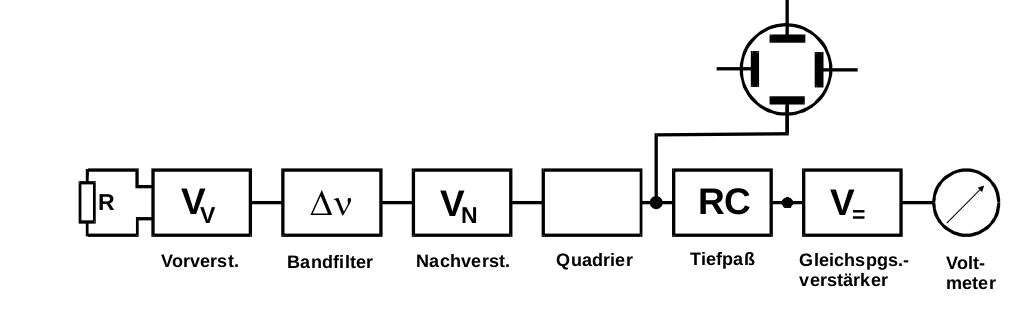
\includegraphics[width=0.8\linewidth,height=0.5\textheight,keepaspectratio]{bilder/EinfacheSchaltung.png}
	\caption{Schematisch Darstellung der Messung des Widerstandsrauschens mit der einfachen Schaltung \cite{Anl}}
	\label{FIG:EinfacheSchaltung}
\end{figure}

Gemäß der Nyquist-Beziehung \eqref{eqn:Nyquist} findet man unter Berücksichtigung der Verstärker für die Ausgangsspannung $U^2_{\textrm{a}}$ in Abhängigkeit des Spannungsabfalls am Widerstand $\overline{U_{\textrm{R}}}$

\begin{align}
U^2_{\textrm{a}} = V_{=}V_{\textrm{V}}^2V_{\textrm{N}}^2\overline{U_{\textrm{R}}} = 4kTR\Delta\nu V_{=}V_{\textrm{V}}^2V_{\textrm{N}}^2 \;,
\end{align}

wobei $V_{=}V_{\textrm{V}}^2V_{\textrm{N}}$ als Apparaturkonstante im Rahmen von Eichmessungen mit einem Sinussignal bestimmt werden kann. Dazu wird ein Abschwächer $V_{\textrm{A}}$ zum Schutz der Verstärkungsaparatur verwendet. Zusätzlich wird das Eigenrauschen der Apparatur betrachtet, indem es mit einem $0\;\Omega$ Abschluss vermessen wird.

\subsubsection{Messung mit der Korrelator Schaltung}
Bei Untersuchungen mit hoher Verstärkung stellt das Eigenrauschen der Verstärker eine Ungenauigkeit dar, die man unter Ausnutzung der Unkorreliertheit des Eigenrauschens zweier Verstärker reduzieren kann. Gemäß Abbildung \ref{FIG:KorrelatorSchaltung} wird die, an den beiden zu untersuchenden Widerständen, zu messende Spannung über jeweils zwei getrennte Vorverstärker, Bandfilter und Nachverstärker verstärkt. Anschließend werden beide Leitungsarme zusammengeführt und miteinander multipliziert, auf einen Tiefpass gegeben und in einem Gleichspannungsverstärker noch einmal nachverstärkt.

\begin{figure}[htbp]
	\centering
	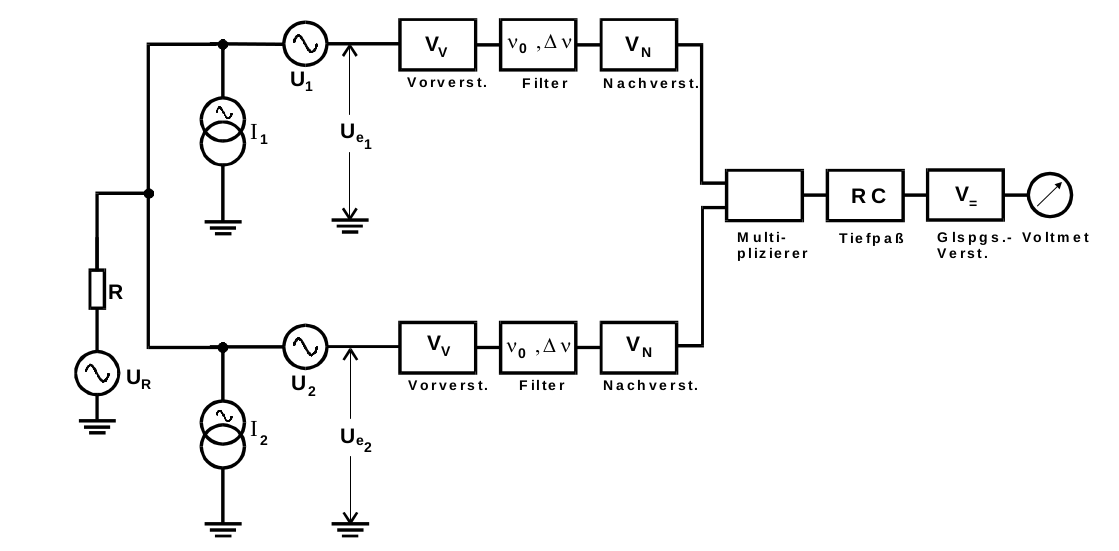
\includegraphics[width=0.8\linewidth,height=0.5\textheight,keepaspectratio]{bilder/KorrelatorSchaltung.png}
	\caption{Schematisch Darstellung der Messung des Widerstandsrauschens mit der Korrelator Schaltung \cite{Anl}}
	\label{FIG:KorrelatorSchaltung}
\end{figure}

Man erhält dann

\begin{align}
U^2_{\textrm{a, Kor}} = V_{\textrm{Ges}}^2 \overline{U_{\textrm{R}}} \;,
\end{align}

wobei wieder $V_{\textrm{Ges}}^2$ durch Kalibrationsmessungen und das Eigenrauschen durch Vermessung von einem $0\;\Omega$ Abschluss ermittelt wird. Zusätzlich wird die Rauschzahl $F$

\begin{align}
F(\nu, Z) = \frac{\overline{U^2_{\textrm{a}}}(Z)}{4kT \textrm{Re}(Z) \Delta\nu V_{\textrm{Ges}}^2}
\label{eq:F}
\end{align}

für $Z = 500\; \Omega$ ermittelt. Die Rauschzahl ist idealerweise $F = 1$ und kann auch in Dezibel gemäß

\begin{align}
F[ \textrm{db} ] = 10 \textrm{log}_{10}(f)
\end{align}

angegeben werden.

\subsection{Stromrauschen an Elektronenröhren}
\subsubsection{Messung des Schrot-Rauschens an einer Reinmetallkathode}
Der Schroteffekt wird mit Hilfe einer Reinmetallkathode mit einer Beschaltung gemäß Abbildung \ref{FIG:SchrotRauschquelle} vermessen. Zuerst werden zwei Kennlinien bei zwei verschiedenen Heizströmen aufgenommen, um sicherzustellen, dass die Elektronenröhre im Sättigungsbereich betrieben wird, da nur dann die Annahmen aus Abschnitt \ref{sec:Schrotrauschen} annähernd zutreffen. Über eine Feinregelung wird der Anodenstrom während der Versuchsdurchführung konstant gehalten.

\begin{figure}[htbp]
	\centering
	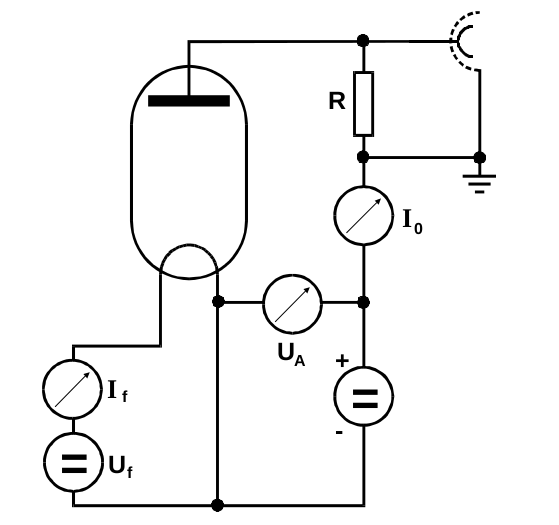
\includegraphics[width=0.5\linewidth,height=0.5\textheight,keepaspectratio]{bilder/SchrotRauschquelle.png}
	\caption{Schematisch Darstellung der Beschaltung der Schrotrauschquelle \cite{Anl}}
	\label{FIG:SchrotRauschquelle}
\end{figure}

Die Verstärkung erfolgt gemäß Abbildung \ref{FIG:SchrotRauschenMessaufbau}, wobei für Frequenzen unterhalb von $100\;$ kHz ein Selektivverstärker und für darüber ein Bandfilter verwendet wird.

\begin{figure}[htbp]
	\centering
	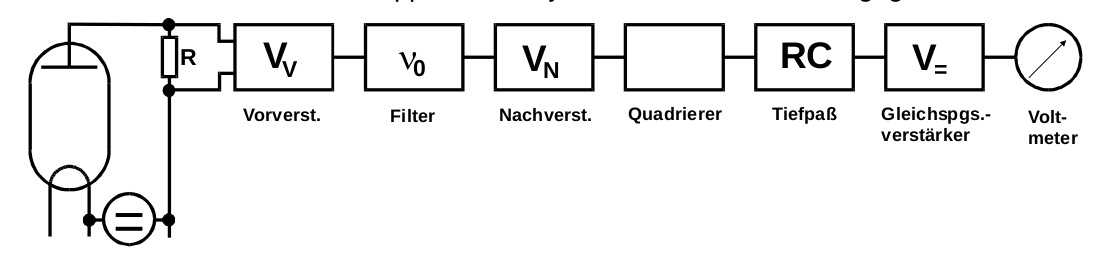
\includegraphics[width=0.7\linewidth,height=0.5\textheight,keepaspectratio]{bilder/SchrotRauschenMessaufbau.png}
	\caption{Schematisch Darstellung des Aufbaus zur Messung des Schroteffekts und des Funkeleffekts \cite{Anl}}
	\label{FIG:SchrotRauschenMessaufbau}
\end{figure}

\subsubsection{Messung des Funkeleffekts an einer Oxidkathode}
Das Rauschspektrum zur Untersuchung des Funkeleffektes wird mit Hilfe einer Oxidkathode mit dem selben Aufbau wie im vorherigen Abschnitt gemäß Abbildung \ref{FIG:SchrotRauschenMessaufbau} durchgeführt.


\section{Auswertung}
\subsection{Eigenrauschen}
Zunächst muss das Eigenrauschen der Apparatur bei verschiedenen Gain Einstellungen bestimmt werden, da alle folgenden Messungen um diesen Wert korrigiert werden müssen.

Dazu wurde ein \SI{0}{\ohm} Widerstand an den Eingang angeschlossen und anschließend das Rauschspannungsquadrat $U_0^2$ bei allen Nachverstärkungsstufen $(V_N)$ gemessen. Die Ergebnisse der Messungen stehen in den Tabellen \ref{tab:eigenRauschen_norm} und \ref{tab:eigenRauschen_korr}.

\begin{table}[h]
	\centering
	\begin{subtable}[c]{0.3\textwidth}
		\begin{tabular}{lS}
			{$V_N$} & {$U_0^2$ [\si{\milli\volt}]}\\
			\toprule
			1	& 4.0\\
			2	& 4.0\\
			5	& 4.0\\
			10	& 4.0\\
			20	& 4.0\\
			50	& 4.0\\
			100	& 3.6\\
			200	& 1.0\\
			500	& 12.0\\
			1000& 55.6
		\end{tabular}
		\caption{Normale Schaltung}
		\label{tab:eigenRauschen_norm}
	\end{subtable}%
	\hspace{1cm}%
	\begin{subtable}[c]{0.3\textwidth}
		\begin{tabular}{lS}
			{$V_N$} & {$U_0^2$ [\si{\milli\volt}]}\\
			\toprule
			1	&-11.1 \\
			2	&-10.9 \\
			5	&-11.0 \\
			10	&-11.1 \\
			20	&-11.0 \\
			50	&-10.8 \\
			100	&-10.2 \\
			200	&-9.8 \\
			500	&0.5 \\
			1000	&53.0
		\end{tabular}
		\caption{Korrelationsschaltung}
		\label{tab:eigenRauschen_korr}
	\end{subtable}
	\caption{Eigenrauschen der Apparatur bei den beiden verwendeten Aufbauten.}
	\label{tab:eigenRauschen}
\end{table}

\subsection{Eichung}
Bevor die eigentlichen Messungen durchgeführt werden können, muss die Apparatur zudem geeicht werden.

Ein Sinuswellengenerator wird mit einer Amplitude von \SI{175}{\milli\volt} an den Eingang angeschlossen und durch einen Abschwächer um den Faktor 1000 reduziert. Der Bandpass wird so eingestellt, dass er nur Frequenzen im Bereich von \SIrange{10}{20}{\kilo\hertz} passieren lässt und die Nachverstärkung wird so eingestellt, dass die Spannungen mit genug Nachkommastellen im Millivoltbereich abgelesen werden kann. Die Messwerte stehen in Tabelle \ref{tab:sin1} und eine graphische Darstellung der mittels Gleichung \ref{eq:eta} umgeformten Spannung $\eta(\nu)$ ist in Abbildung \ref{fig:eichmessung} zusehen.
\begin{align}
	\eta(\nu) &= \frac{\overline{U^2_a}}{V_\text{ges}U^2_e}
	\label{eq:eta}\\
	V_\text{ges} &= V_V^2V_S^2V_N^2V_=
\end{align}
\begin{align*}
	V_V &= \text{Vorverstärkung}, V_S = \text{Selektivverstärkung}, V_N = \text{Nachverstärkung},\\ V_=&=\text{Gleichspannungsverstärkung}
\end{align*}
\begin{figure}[h]
	\includegraphics[height=8.5cm]{../auswertung/results/sin.pdf}
	\caption{Messwerte aus der Eichmessung. Der Bandpass wurde auf das Intervall \SI{10}{\kilo\hertz} - \SI{20}{\kilo\hertz} eingestellt.}
	\label{fig:eichmessung}
\end{figure}


Um die Apparaturkonstante
\begin{align}
	\Delta\nu &= \int_0^\infty \eta(\nu)\ d\nu
\end{align}
zu bestimmen, wird die Integralfläche mittels Trapezregel bestimmt.
Damit ergibt sich für die normale Schaltung:
\begin{align}
\Delta\nu = (\input{../auswertung/results/sin1_DeltaNu.fit})\, \si{\hertz}
\end{align}

Die Fehler wurde mittels des Restgliedes der Trapezregel abgeschätzt:
\begin{align}
	\textbar R(f)\textbar = \frac{b-a}{12}h^2\text{max}\left(f''(x)\right)
	\label{eq:restglied}
\end{align}
Mit diesem Wert kann nun die Rauschzahl der Schaltung berechnet werden. 
\begin{align*}
	T &= \SI{293}{\kelvin}\\
	V^2_\text{ges} &= V_=V^2_VV^2_N = 10^{13}\, \si{\volt}\\
	U^2(500\Omega) &= (706.0\pm 14.1)\,{\milli\volt}\\
	F(500\Omega, \Delta\nu) &= \frac{U^2(500)}{4k_\text{B} \cdot \SI{293}{\kelvin} \cdot \SI{500}{\ohm} \cdot \Delta\nu \cdot V^2_\text{ges}} = \input{../auswertung/results/rausch1.fit}
\end{align*}
Der Fehler für die Spannung $U^2$ wurde dazu mit $2\%$ abgeschätzt.\\

Um die Boltzmann-Konstante $k_B$ zu berechnen, wird der Sinusgenerator durch einen Variablen Widerstand ausgetauscht und die Rauschspannung gegen den Widerstand aufgetragen (siehe Tabellen \ref{tab:wid1_norm} und \ref{tab:wid2_norm}). Mittels linearer Regression, kann dann über die Nyquist-Beziehung (Gleichung \ref{eqn:Nyquist}) $k_B$ bestimmt werden. Die graphische Darstellung der Messwerte ist in den Abbildungen \ref{fig:thermRauschen1} und \ref{fig:thermRauschen2} zu finden.\\

Ergebnis der Regression mit dem \SI{1000}{\ohm} Widerstand.
\begin{align*}
	m &= \input{../auswertung/results/wid1_m.fit}\,\si{\volt\per\ohm}\\
	b &= \input{../auswertung/results/wid1_b.fit}\,\volt\\
	k_{B,1000\,\Omega} &= \frac{m}{4T\Delta\nu} =\input{../auswertung/results/wid1_kb.fit}\,\si{\joule\per\kelvin}\\
\end{align*}

Ergebnis der Regression mit dem \SI{100}{\kilo\ohm} Widerstand.
\begin{align*}
m &= \input{../auswertung/results/wid2_m.fit}\,\si{\volt\per\ohm}\\
b &= \input{../auswertung/results/wid2_b.fit}\,\volt\\
k_{B,100\,\Omega} &= \input{../auswertung/results/wid2_kb.fit}\,\si{\joule\per\kelvin}
\end{align*}

\begin{figure}[H]
	\includegraphics[width=\textwidth]{../auswertung/results/wid1.pdf}
	\caption{Thermisches Rauschen mit dem \SI{1000}{\ohm} Widerstand.}
	\label{fig:thermRauschen1}
\end{figure}

\begin{figure}[H]
	\includegraphics[width=\textwidth]{../auswertung/results/wid2.pdf}
	\caption{Thermisches Rauschen mit dem \SI{100}{\kilo\ohm} Widerstand.}
	\label{fig:thermRauschen2}
\end{figure}


\subsection{Korrelator-Schaltung}
Nun wird die gleiche Rechnung für die Korrelatorschaltung wiederholt. Die Verstärkungsfaktoren sind dabei bis auf einen zusätzlichen Faktor 10 durch den Selektivverstärker identisch zur vorherigen Schaltung.

Begonnen wird mit der Eichung. Mittels Trapezregel werden die Datenpunkte aus Tabelle \ref{tab:sin2} integriert und in Abbildung \ref{fig:eichmessung_korrel} dargestellt. Der Fehler übersteigt den Messwert um mehrere Größenordnungen, da für die Restgliedabschätzung (Gleichung \ref{eq:restglied}) die zweite Ableitung verwendet wird und im Bereich des Peaks zu wenige Messungen durchgeführt wurden. Für alle folgenden Rechnungen wird daher der Fehler ignoriert.
\begin{align}
\Delta\nu= (\input{../auswertung/results/sin2_DeltaNu.fit})\,\si{\hertz}
\end{align}

Auch von der Korrelatorschaltung wird die Rauschzahl nach Gleichung \ref{eq:F} bestimmt

\begin{align*}
T &= \SI{293}{\kelvin}\\
V^2_\text{ges} &= V_=V^2_VV^2_NV_S^2 = 10^{15}\, \si{\volt}\\
U^2(500\Omega) &= (625.0\pm 12.5)\,{\milli\volt}\\
F(500\Omega, \Delta\nu) &= \input{../auswertung/results/rausch2.fit}
\end{align*}

\begin{figure}[htbp]
	\centering
	\includegraphics[height=8.5cm]{../auswertung/results/sin_korrel.pdf}
	\caption{Messwerte aus der Eichmessung der Korrelationsschaltung. Die Selektivverstärker wurden auf \SI{15}{\kilo\Hz} eingeregelt.}
	\label{fig:eichmessung_korrel}
\end{figure}

und mittels Nyquist-Beziehung die Boltzmann Konstante $k_\text{B}$ ermittelt.

Bei der Korrelatorschaltung lässt sich die Rauschspannung zudem durch folgende Formel ausdrücken:
\begin{align}
	U^2_a = \frac{U_e^2}{Q^2}\frac{1}{\eta^2 + \eta^{-2} + Q^{-2} -2} \qquad \qquad ;\eta = \frac{\nu}{\nu_0}
\end{align}
Mit dem least-square Verfahren wurde die Formel an die Messpunkte aus Tabelle \ref{tab:sin2} angenähert (Abbildung \ref{fig:eichmessung_korrel}). Bei der grünen Kurve wurden alle drei Parameter durch den Algorithmus ermittelt und bei der roten Kurve wurden die Parameter $Q=10$ und $V_E=0.175\,\si{mV}$ gesetzt, was der Konfiguration des Experimentes entspricht.
\begin{align}
	\nu_0 &= (\input{../auswertung/results/sin2_nu0.fit}) \,\hertz\\
	Q &= (\input{../auswertung/results/sin2_Q.fit})\\
	V_E &= \input{../auswertung/results/sin2_U.fit}\, \si{\volt}
\end{align}

Der Sinusgenerator wird durch die Widerstände ersetzt:\\
Ergebnis der Regression mit dem \SI{1000}{\ohm} Widerstand und den Messwerten aus \mbox{Tabelle \ref{tab:wid1_korrel}}.
\begin{align*}
m &= \input{../auswertung/results/wid1_korrel_m.fit}\,\si{\volt\per\ohm}\\
b &= \input{../auswertung/results/wid1_korrel_b.fit}\,\volt\\
k_{B,1000\,\Omega} &= \frac{m}{4T\Delta\nu} =\input{../auswertung/results/wid1_korrel_kb.fit}\,\si{\joule\per\kelvin}\\
\end{align*}

Ergebnis der Regression mit dem \SI{100}{\kilo\ohm} Widerstand und den Messwerten aus \mbox{Tabelle \ref{tab:wid2_korrel}}.
\begin{align*}
m &= \input{../auswertung/results/wid2_korrel_m.fit}\,\si{\volt\per\ohm}\\
b &= \input{../auswertung/results/wid2_korrel_b.fit}\,\si{\volt}\\
k_{B,100\,k\Omega} &= \input{../auswertung/results/wid2_korrel_kb.fit}\,\si{\joule\per\kelvin}
\end{align*}

\begin{figure}[htbp]
	\includegraphics[height=8.5cm]{../auswertung/results/wid1_korrel.pdf}
	\caption{Thermisches Rauschen mit dem \SI{1000}{\ohm} Widerstand.}
	\label{fig:thermRauschen1}
\end{figure}

\begin{figure}[htbp]
	\includegraphics[height=8.5cm]{../auswertung/results/wid2_korrel.pdf}
	\caption{Thermisches Rauschen mit dem \SI{100}{\kilo\ohm} Widerstand.}
	\label{fig:thermRauschen2}
\end{figure}

\subsection{Reinmetall-Kathode}
\begin{figure}[htbp]
	\includegraphics[height=8.5cm]{../auswertung/results/kathRein_sat.pdf}
	\caption{Kennlinien der Reinkathode aufgenommen bei zwei verschiedenen Heizströmen.}
	\label{fig:kennlinie}
\end{figure}
Zunächst werden Kennlinien der Reinmetall-Kathode aufgenommen, damit sichergestellt werden kann, dass die Kathode bei der Datennahme im Sättigungsbereich betrieben wird. Die Messwerte sind in Tabelle \ref{tab:kennlinien} und Abbildung \ref{fig:kennlinie} dargestellt. Für alle folgenden Messungen wird eine Spannung von \SI{150}{\volt} verwendet.

Um die Elementarladung $e_0$ zu berechnen, kann die Schottky-Beziehung zu
\begin{align}
	\overline{U_a^2} = \frac{2e_0 \ \Delta\nu}{R} I_0
	\label{eq:schottKey}
\end{align}
umgestellt werden. Misst man die Rauschspannung der Reinmetallkathode in Abhängigkeit vom Anodenstrom, so erhält man die in Tabelle \ref{tab:e0} und Abbildung \ref{fig:e0} dargestellten Messwerte und kann mittels linearer Regression über die Geradensteigung die Elementarladung $e_0$ bestimmt werden. $\Delta\nu$ der Schaltung war dabei \SI{10}{\kilo\hertz} und der Widerstand R der Kathode betrug \SI{4680}{\ohm}.
\begin{figure}[h]
	\includegraphics[height=8.5cm]{../auswertung/results/rein_e0.pdf}
	\caption{Rauschspannung der Reinmetallkathode in Abhängigkeit vom Anodenstrom. Durch lineare Regression lässt sich $e_0$ ermitteln.}
	\label{fig:e0}
\end{figure}
\begin{align}
	m &= \input{../auswertung/results/rein_m.fit}\, \frac{\si{\coulomb}}{\si{\second}}\\
	e_0 &= \input{../auswertung/results/rein_e0.fit}\, \si{\coulomb}
\end{align}
Die lineare Regression wurde mittels Gleichung \ref{eq:schottKey} durchgeführt.\\

Das Rauschspektrum der Reinmetall-Kathode ist in Abbildung \ref{fig:rauschspektrum} dargestellt und die Messwerte stehen in Tabelle \ref{tab:rein_rauschen}. Dieses wird ermittelt gemäß:
\begin{align}
	W_\text{Sch}(\nu) = \frac{\overline{U^2}(\nu)}{R^2 \Delta\nu(\nu)} 
\end{align}
\begin{figure}[h]
	\includegraphics[height=8.5cm]{../auswertung/results/rein_rausch.pdf}
	\caption{Rauschspektrum der Reinmetallkathode. Die Messpunkte wurden entsprechend ihrer Zugehörigkeit zum Schrot- oder Funkelrauschen eingefärbt und die Werte aus dem Funkelrauschen wurden um das Schrotrauschen korrigiert. Die Fitfunktion ist in der doppelt logarithmischen Darstellung eine Gerade.}
	\label{fig:rauschspektrum}
\end{figure}
Aus dem Graphen lässt sich für den Schrotanteil ablesen:
\begin{align}
	W_\text{Sch} = \input{../auswertung/results/rein_schrot_W.fit}\,\si{\ampere^2\second}
\end{align}
und für den Funkelanteil:
\begin{align}
F = \input{../auswertung/results/rein_funkel_F.fit}
\end{align}

\subsection{Oxidkathode}
Die selbe Messung wird bei der Oxidmetall-Kathode wiederholt.

In Abbildung \ref{fig:rauschspektrum_oxid} ist ihr Rauschspektrum zu sehen, die zugehörigen Messwerte sind in Tabelle \ref{tab:oxid_rauschen} aufgeführt.
Aus dem Graphen erhält man:
\begin{align}
W_\text{Sch} = \input{../auswertung/results/oxid_schrot_W.fit}\,\si{\ampere^2\second}
\end{align}
und für den Funkelanteil:
\begin{align}
F = \input{../auswertung/results/oxid_funkel_F.fit}
\end{align}

\begin{figure}[h]
	\includegraphics[height=8.5cm]{../auswertung/results/oxid_rausch.pdf}
	\caption{Rauschspektrum der Oxidmetall-Kathode. Die Messpunkte wurden entsprechend ihrer Zugehörigkeit zum Schrot- oder Funkelrauschen eingefärbt und die Werte aus dem Funkelrauschen wurden um das Schrotrauschen korrigiert. Die Fitfunktion ist in der doppelt logarithmischen Darstellung eine Gerade.}
	\label{fig:rauschspektrum_oxid}
\end{figure}

\section{Diskussion}
\subsection{Bestimmung der Boltzmannkonstante}
Mit Hilfe des aufgebauten Rauschspektrometers wurde die Boltzmann-Konstante anhand des thermischen Rauschens in zwei Widerständen berechnet. Zunächst wurde die Konstante durch die normale Schaltung bestimmt und anschließend nochmal durch eine Korrelatorschaltung mit einer höheren Präzision.

Die Messungen ergaben:
\begin{table}[H]
\begin{tabular}{lcc}
	& \SI{1000}{\ohm} & \SI{100}{\kilo\ohm}\\
	\cmidrule{2-3}
	Normal $\left[\frac{\joule}{\kelvin}\right]$ & $\input{../auswertung/results/wid1_kb.fit}$ & $\input{../auswertung/results/wid2_kb.fit}$\\
	Korrelator $\left[\frac{\joule}{\kelvin}\right]$& $\input{../auswertung/results/wid1_korrel_kb.fit}$ & $\input{../auswertung/results/wid2_korrel_kb.fit}$\\
	\cmidrule{2-3}
	Normal & $91.3\%$ & $60.8\,\%$\\
	Korrelator & $176.1\%$ & $140.6\,\%$
\end{tabular}
\caption{Ergebnisse der $K_\text{B}$ Messung}
\end{table}

Im Vergleich mit dem Literaturwert von $K_\text{B} = 1.381 \cdot 10^{-23}$ \si{\joule\per\kelvin} wird ersichtlich, dass die berechneten Werte für den \SI{100}{\kilo\ohm} Widerstand näher am Literaturwert liegen als beim \SI{1000}{\ohm} Widerstand und die normale Schaltung ein besseres Ergebnis als die Korrelatorschaltung erbrachte.
\subsection{Bestimmung der Elementarladung}
Die gemessene Elementarladung $ \input{../auswertung/results/rein_e0.fit}\, \si{\coulomb}$ weicht um eine halbe Größenordnung vom Literaturwert $1.602\cdot 10^{-19}\,\si{\coulomb}$ ab. Dass der Fit ebenso wie bei der Messung der Boltzmannkonstanten einen sehr geringen Fehler aufweist, deutet auf einen Systematischen Fehler bei der Messung hin.
\subsection{Untersuchung der Rauschspektren}
Die Messung des Schrotrauschens ergab bei der Oxidmetallkathode einen Wert von
\begin{align*}
W_\text{Oxid} = \input{../auswertung/results/oxid_schrot_W.fit}\,\si{\ampere^2\second}
\end{align*}
und bei der Reinmetallkathode:
\begin{align*}
W_\text{Rein} = \input{../auswertung/results/rein_schrot_W.fit}\,\si{\ampere^2\second}
\end{align*}
Mittels
\begin{align*}
W_\text{Oxid}(\nu) = 2e_0I_0 &= 2\cdot 1.602\cdot10^{-19}\cdot 0.001 \\
&\approx 3.2\cdot10^{-22}\,\si{\ampere^2\second}\\
W_\text{Rein}(\nu) = 2e_0I_0 &= 2\cdot 1.602\cdot10^{-19}\cdot 1.175 \cdot10^{-3} \\
&\approx 3.8\cdot10^{-22}\,\si{\ampere^2\second}
\end{align*}
lassen sich die theoretisch erwarteten Werte abschätzen. Das Schrotrauschen der Oxidkathode weicht um $62.9\%$ vom Erwartungswert ab. Das Rauschen der Reinmetallkathode weicht dagegen nur um $1.8\%$ vom Theoriewert ab und liegt innerhalb der Standardabweichung.\\

Bei der Reinmetall-Kathode wurde nach Abzug des Schrotrauschanteils ein Funkelkoeffizient von
\begin{align*}
	F_\text{Rein} = \input{../auswertung/results/rein_funkel_F.fit}
\end{align*}
gemessen. Dieser weicht stark vom erwarteten Wert $F=-1$ ab. Die Messung an der Oxidkathode ergab dagegen einen sehr guten Wert, der mit
\begin{align*}
F_\text{Oxid} = \input{../auswertung/results/oxid_funkel_F.fit}
\end{align*}
noch innerhalb des Fehlerintervals liegt.

\section{Tabellen}
\begin{table}
	\input{../auswertung/latex_sin1}
	\caption{Messung mit dem Sinusgenerator für die Kalibration - normale Schaltung}
	\label{tab:sin1}
\end{table}
\begin{table}
	\input{../auswertung/latex_sin2}
	\caption{Messung mit dem Sinusgenerator für die Kalibration -  Korrelationsschaltung}
	\label{tab:sin2}
\end{table}
\begin{table}
	\input{../auswertung/latex_wid1}
	\caption{Messung mit dem $1000\,\ohm$ Widerstand  - normale Schaltung}
	\label{tab:wid1_norm}
\end{table}
\begin{table}
	\input{../auswertung/latex_wid2}
	\caption{Messung mit dem $100\,k\ohm$ Widerstand  - normale Schaltung}
	\label{tab:wid2_norm}
\end{table}
\begin{table}
	\input{../auswertung/latex_wid1_korrel}
	\caption{Messung mit dem $1000\,\ohm$ Widerstand  - Korrelationsschaltung}
	\label{tab:wid1_korrel}
\end{table}
\begin{table}
	\input{../auswertung/latex_wid2_korrel}
	\caption{Messung mit dem $100\,k\ohm$ Widerstand  - Korrelationsschaltung}
	\label{tab:wid2_korrel}
\end{table}
\begin{table}
	\input{../auswertung/latex_kennlinie}
	\caption{Kennlinien der Reinmetallkathode. Heizströme bei \SI{0.9}{\milli\ampere} und \SI{0.925}{\milli\ampere}. Anodenströme in Abhängigkeit von der Beschleunigungsspannung $U_B$.}
	\label{tab:kennlinien}
\end{table}
\begin{table}
	\input{../auswertung/latex_rein_e0}
	\caption{Rauschspannung der Reinmetallkathode. Heizstrom beträgt \SI{1.0}{\milli\ampere}.}
	\label{tab:e0}
\end{table}
\begin{table}
	\input{../auswertung/latex_rein_rauschen}
	\caption{Rauschspektrum der Reinmetallkathode in Abhängigkeit der Frequenz. $\overline{U^2}$ ist die gemessene Rauschspannung und $\sigma$ ihre Standardabweichung.}
	\label{tab:rein_rauschen}
\end{table}
\begin{table}
	\input{../auswertung/latex_oxid_rauschen}
	\caption{Rauschspektrum der Oxidmetallkathode in Abhängigkeit der Frequenz. $\overline{U^2}$ ist die gemessene Rauschspannung und $\sigma$ ihre Standardabweichung.}
	\label{tab:oxid_rauschen}
\end{table}

\clearpage
\begin{thebibliography}{WissOnl}
	\bibitem{Anl} TU Dortmund Versuchsanleitung zu Versuch Nr.57 (abgerufen am 20.4.2014) \url{http://129.217.224.2/HOMEPAGE/PHYSIKER/BACHELOR/FP/SKRIPT/V57.pdf}
\end{thebibliography}

% ========================================
%	Literaturverzeichnis
% ========================================

%\bibliographystyle{plainnat}			% Bibliographie-Style auswählen
%\bibliography{BIBDATEI}			% Literaturverzeichnis

% ========================================
%	Das Dokument endent
% ========================================
\end{document}
